\documentclass[twoside,11pt,a4paper]{article}

% packages %%%%%%%%%%%%%%%%%%%%%%%%%%%%%%%%%%%%%%%%%%%%%%%%%%%%%%%%%%%%%%%%%%%%
\usepackage{graphicx,curves,float,rotating}

\usepackage{amsmath, amssymb, latexsym}  % math stuff
\usepackage{amsopn}                             % um mathe operatoren zu deklarieren
%\usepackage[ngerman]{babel}                     % otherwise use british or american
\usepackage[american]{babel}
\usepackage{theorem}                            % instead of \usepackage{amsthm}
\usepackage{dcolumn}
\usepackage{hyperref}
\usepackage[outdir=./]{epstopdf}
\epstopdfsetup{outdir=./}

% @ environment %%%%%%%%%%%%%%%%%%%%%%%%%%%%%%%%%%%%%%%%%%%%%%%%%%%%%%%%%%%%%%%%
\usepackage{xspace}                             % context sensitive space after macros
\makeatletter 
\DeclareRobustCommand\onedot{\futurelet\@let@token\@onedot}
\def\@onedot{\ifx\@let@token.\else.\null\fi\xspace}
\def\eg{{e.g}\onedot} \def\Eg{{E.g}\onedot}
\def\ie{{i.e}\onedot} \def\Ie{{I.e}\onedot}
\def\cf{{c.f}\onedot} \def\Cf{{C.f}\onedot}
\def\etc{{etc}\onedot} \def\vs{{vs}\onedot} 
\def\wrt{w.r.t\onedot} \def\dof{d.o.f\onedot}
\def\etal{{et al}\onedot}
\def\zB{z.B\onedot} \def\ZB{Z.B\onedot}
\def\dh{d.h\onedot} \def\Dh{D.h\onedot}
% %%%%%%%%%%%%%%%%%%%%%%%%%%%%%%%%%%%%%%%%%%%%%%%%%%%%%%%%%%%%%%%%%%%%%%%%%%%%%%%


\newcommand*{\Frac}[2]{\frac{\displaystyle #1}{\displaystyle #2}}
\newlength{\textwd}
\newlength{\oddsidemargintmp}
\newlength{\evensidemargintmp}
\newcommand*{\hspaceof}[2]{\settowidth{\textwd}{#1}\mbox{\hspace{#2\textwd}}}
\newlength{\textht}
\newcommand*{\vspaceof}[3]{\settoheight{\textht}{#1}\mbox{\raisebox{#2\textht}{#3}}}
\newcommand*{\PreserveBackslash}[1]{\let\temp=\\#1\let\\=\temp}

\newenvironment{deflist}[1][\quad]%
{  \begin{list}{}{%
      \renewcommand{\makelabel}[1]{\textbf{##1}\hfil}%
      \settowidth{\labelwidth}{\textbf{#1}}%
      \setlength{\leftmargin}{\labelwidth}
      \addtolength{\leftmargin}{\labelsep}}}
{  \end{list}}


\newenvironment{Quote}% Definition of Quote
{  \begin{list}{}{%
      \setlength{\rightmargin}{0pt}}
      \item[]\ignorespaces}
{\unskip\end{list}}


\theoremstyle{break}
\theorembodyfont{\itshape}	
\theoremheaderfont{\scshape}

\newtheorem{Cor}{Corollary}
\newtheorem{Def}{Definition}
%\newtheorem{Def}[Cor]{Definition}



\newcolumntype{.}{D{.}{.}{-1}}


\pagestyle{headings}
\textwidth 15cm
\textheight 23cm
\oddsidemargin 1cm
\evensidemargin 0cm
%\parindent 0mm



%%%%%%%%%%%%%%%%%%%%%%%%%%%%%%%%%%%%%%%%%%%%%%%%%%%%%%%%%%%%%%%%%%%%%%%%%%%%%%%
%
%%%%%%%%%%%%%%%%%%%%%%%%%%%%%%%%%%%%%%%%%%%%%%%%%%%%%%%%%%%%%%%%%%%%%%%%%%%%%%%
\begin{document}

\pagestyle{empty}

\begin{center}

    Rheinisch-Westf\"alische Technische Hochschule Aachen \\
    Lehrstuhl f\"ur Informatik 6 \\
    Prof. Dr.-Ing. Hermann Ney\\[6ex]
    Seminar Selected Topics in Human Language Technology and Pattern Recognition in WS 2018\\[12ex]
   
    \LARGE
    \textbf{Neural Network Based Natural Language Understanding} \\[6ex]
    \textit{Simon Berger} \\[6ex]
    \Large
    Matrikelnummer 336 353 \\[6ex]
    \today

    \vfill
    \Large Supervisor: Kazuki Irie
	    
\end{center}

\newpage
\ 
\newpage

%%%%%%%%%%%%%%%%%%%%%%%%%%%%%%%%%%%%%%%%%%%%%%%%%%%%%%%%%%%%%%%%%%%%%%%%%%%%%%%
%
%
%               Inhaltsverzeichnis / Tabellenverzeichnis / Abbildungsverz.
%
%
%
%%%%%%%%%%%%%%%%%%%%%%%%%%%%%%%%%%%%%%%%%%%%%%%%%%%%%%%%%%%%%%%%%%%%%%%%%%%%%%%
\pagestyle{headings}
\tableofcontents
\listoftables
\listoffigures
\newpage
\pagestyle{empty}
\ 
\newpage
\pagestyle{headings}

%%%%%%%%%%%%%%%%%%%%%%%%%%%%%%%%%%%%%%%%%%%%%%%%%%%%%%%%%%%%%%%%%%%%%%%%%%%%%%%
%
%
%               Section 1 - Introduction
%
%
%%%%%%%%%%%%%%%%%%%%%%%%%%%%%%%%%%%%%%%%%%%%%%%%%%%%%%%%%%%%%%%%%%%%%%%%%%%%%%%
\section{Introduction}



%%%%%%%%%%%%%%%%%%%%%%%%%%%%%%%%%%%%%%%%%%%%%%%%%%%%%%%%%%%%%%%%%%%%%%%%%%%%%%%
%
%
%               Section 2 - The task of Natural Language Understanding
%
%
%%%%%%%%%%%%%%%%%%%%%%%%%%%%%%%%%%%%%%%%%%%%%%%%%%%%%%%%%%%%%%%%%%%%%%%%%%%%%%%
\section{The task of Natural Language Understanding}


Natural language understanding (NLU) is a key component in any dialogue-system between human and machine. It consists of the task of \textit{'understanding'} a human utterance given in natural language, i.e. forming a semantic frame that captures the semantic meaning of the utterance that the machine can then use. In figure \ref{fig:pipeline} we see the usual pipeline of handling and responding to a natural language utterance in a dialogue-system.\par

\begin{figure}
	\begin{center}
		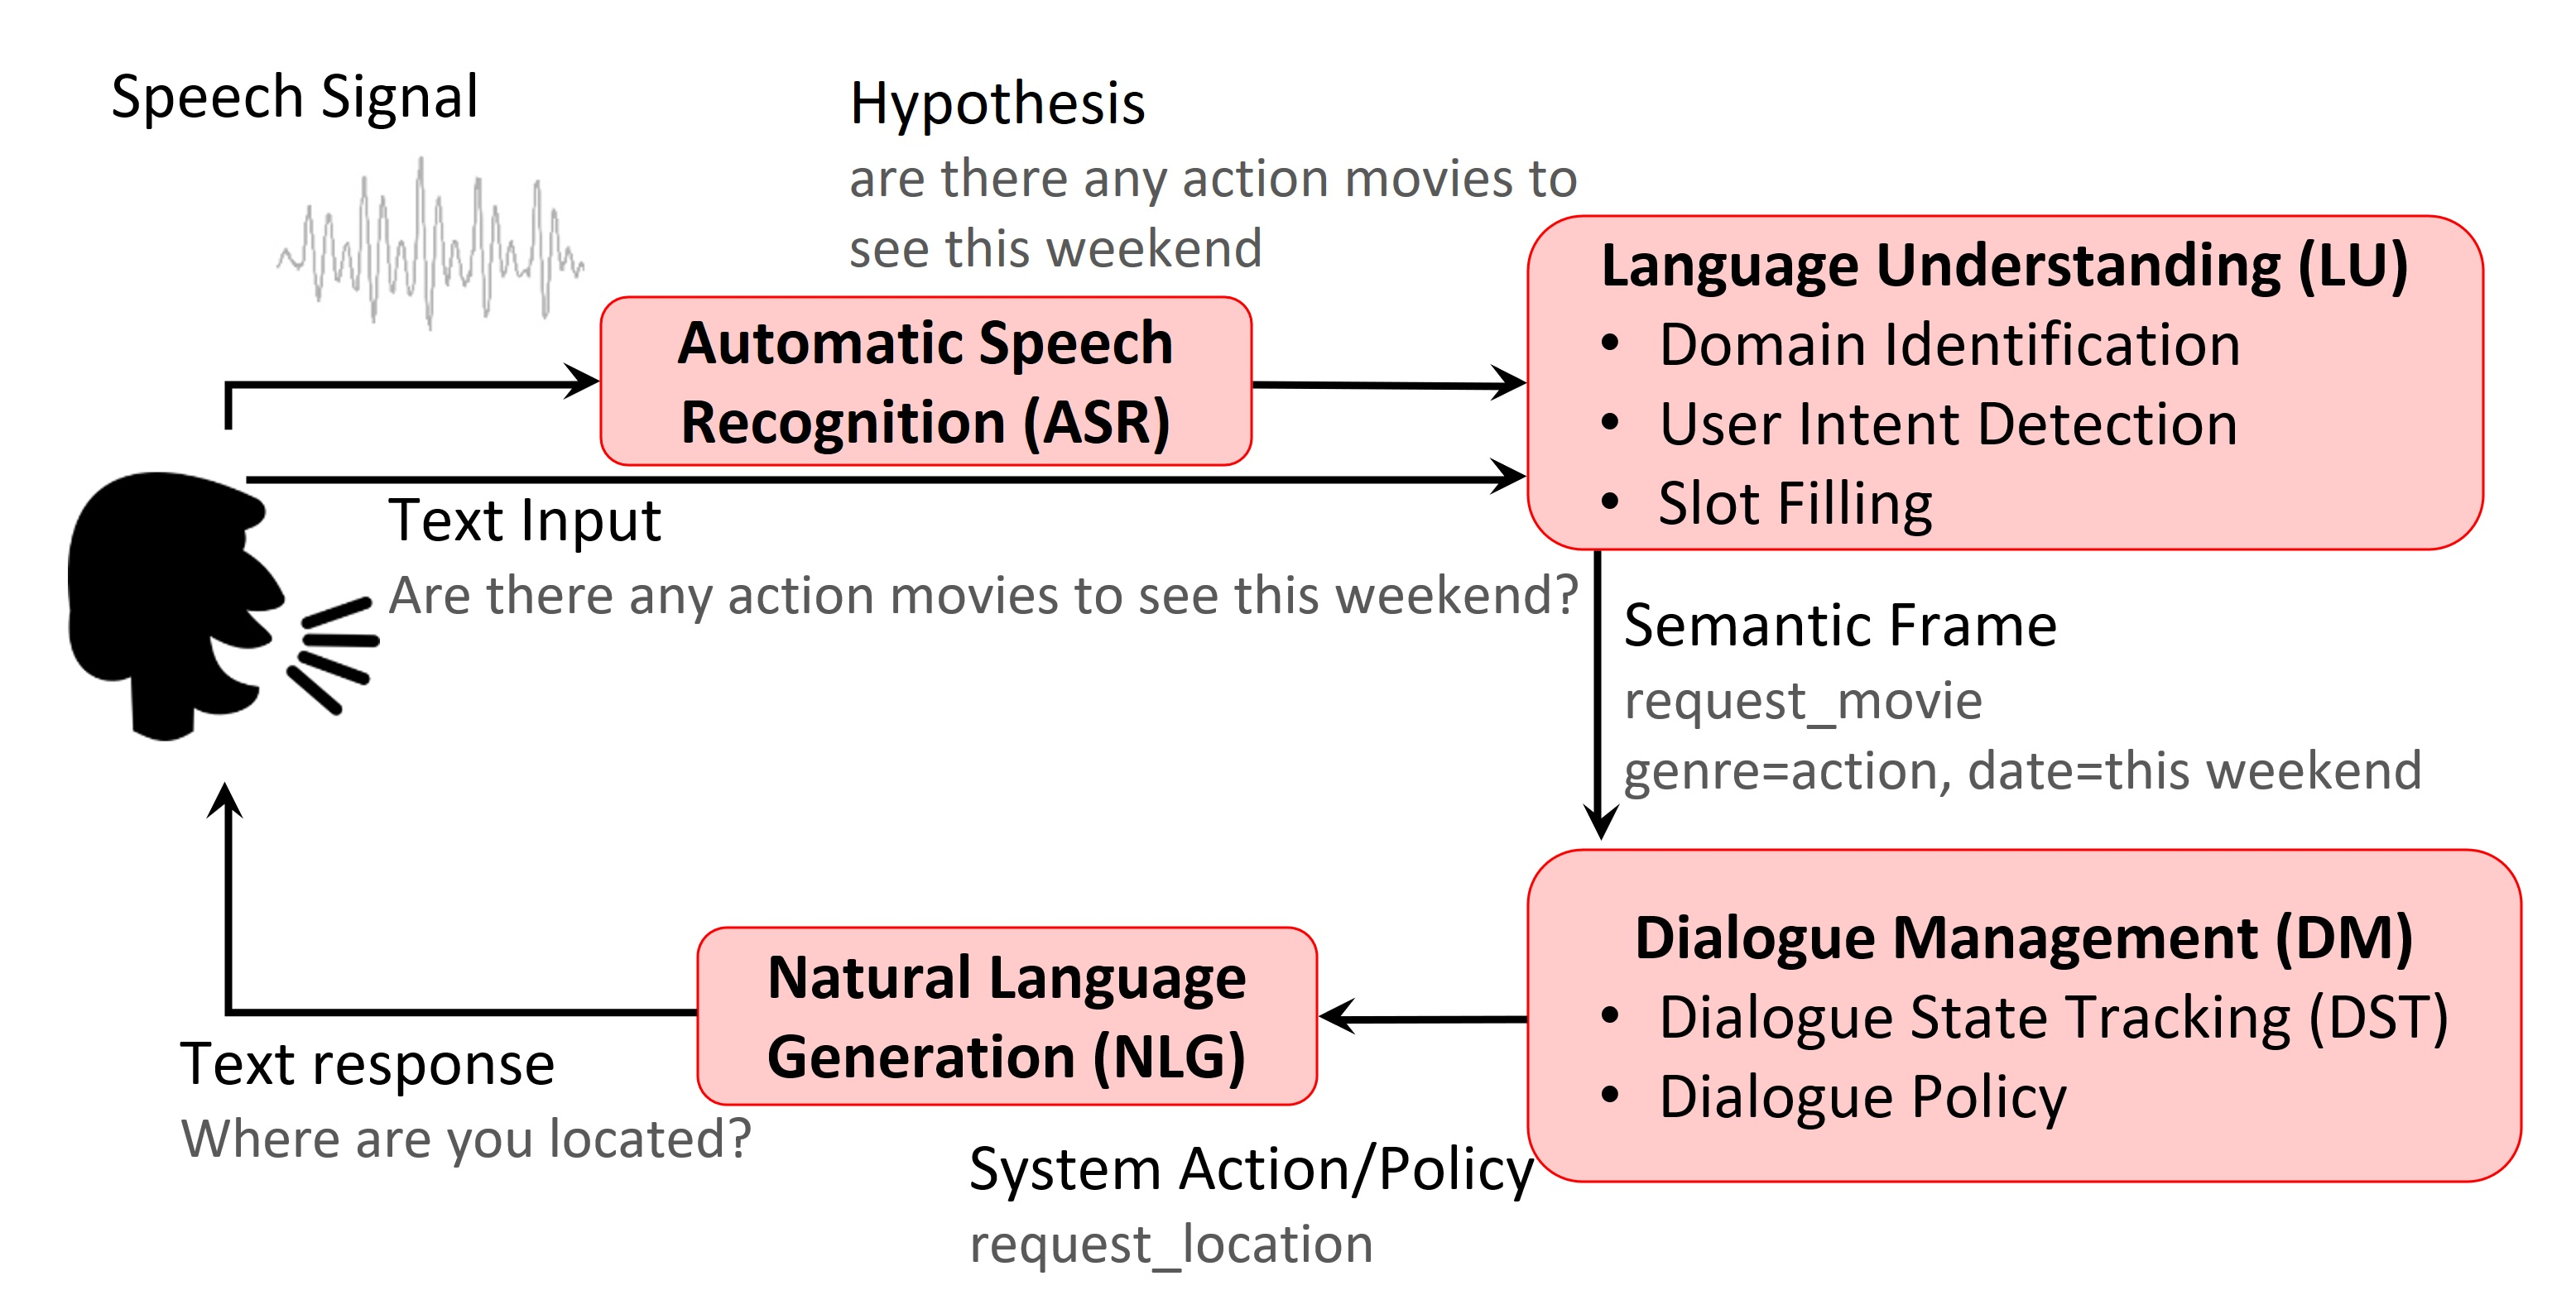
\includegraphics[width=13cm]{pipeline.jpg}
		\caption{Dialogue-system pipeline.}
		Source: https://www.csie.ntu.edu.tw/~yvchen/s105-icb/project.html.
		\label{fig:pipeline}
	\end{center}
\end{figure}

The first step is parsing the raw acoustic-speech signal to written text using an \textit{Automatic Speech Recognition} module. For example the speech-signal might be parsed to the sentence 'Are there any action movies to see this weekend?' If the human query is given in text-form this step can of course be skipped. Afterwards we need to assign semantic meaning to the given text. This is the step of \textit{language understanding} (LU) that we focus on in this article. For example we might classify the domain of the request as \textit{'movies'}, the intent of the query as a \textit{'movie-request'} and extract the genre-information \textit{'action'} and the date-information \textit{'this weekend'}. Using this semantic information the \textit{Dialogue-Manager} (DM) can then decide on the machine's course of action like for example retreiving the sought-after information from the web or requesting additional input from the user. The results then get parsed back into natural language using a \textit{Natural Language Generator} to make them understandable for the user.\par
As indicated in the above example, NLU usually consists of three major subtasks:
\begin{itemize}
	\item Domain Detection: Finding the domain of the request (e.g. \textit{movies, travel, weather}, etc.)
	\item Intent Determination: Determining the domain-specific intent of the user (e.g. \textit{request\_movie, book\_flight, get\_weather}, etc.)
	\item Slot-filling: Extracting associated semantic slots for the intent (e.g. \textit{departure\_city, destination\_city, date}, etc. for intent \textit{book\_flight}).
\end{itemize}
In the following subsections we will describe the mathematical formulation of the three subtasks in detail.

\subsection{Domain Detection task formulation}
Domain detection is typically handled as a semantic utterance classification problem \cite{mesnil:2015} which means that it takes the word-sequence
\[
	x_1^T = (x_1, x_2, \dots, x_T) \in V^T
\]
for some vocabulary-set $V$ as an input and assigns a single domain-label $y^D$ as the output. The possible domain-labels must be designed manually before the classification.

\subsection{Intent Determination task formulation}
Intent determination is similar to domain detection in the sense that is also treated as a semantic utterance classification problem \cite{mesnil:2015}. After the domain was determined, another label $y^I$ must be assigned to the sequence $x_1^T$, representing the domain-specific intent of the user. Again the set of possible intents have to be manually predetermined before performing the classification.

\subsection{Slot Filling task formulation}
\label{subsec:slotfillingtask}
In constrast to the other two subtasks, slot filling is treated as a sequence-labeling problem \cite{mesnil:2013}, which means that we want to assign an output-sequence
\[
	y^S = (y_1^S, y_2^S, \dots, y_T^S)
\]
of semantic slot-labels to the input $x_1^T$. As before the intent-specific possible slots have to be manually crafted before. Since in many cases multiple words can comprise a single semantic entity as for example in \textit{'New York'} or \textit{'President of the United States'}, it is popular to define the slot-labels in an \textit{Inside-Outside-Beginning} (IOB) representation. The first word in a semantic unit has a B-label, each following word belonging to the same semantic slot gets an I-label and each word not belonging to any semantic slot gets an O-label. An example of such slot-labeling in IOB-representation can be found in figure \ref{fig:iob-slots}. 

\begin{figure}[H]
	\begin{center}
		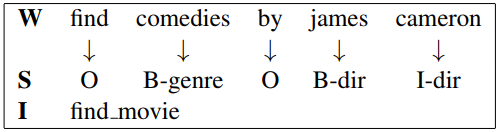
\includegraphics[width=8cm]{iob-slots}
		\caption{Example sentence.}
		An example sentence of words \textbf{W} with slot-labels \textbf{S} in IOB-representation and Intent \textbf{I}. Source: \cite{goo:2018}.
		\label{fig:iob-slots}
	\end{center}
\end{figure}

Here, the words \textit{'find'} and \textit{'by'} don't belong to any semantic slot. The word \textit{'comedies'} belongs to the semantic concept \textit{'genre'} and has a B-tag since it is the first (and only) word in it's chunk. At last, both words \textit{'james'} and \textit{'cameron'} belong to the same semantic concept \textit{'dir'} (director) with the first word \textit{'james'} having a B-tag and the second word \textit{'cameron'} having an I-tag.

%%%%%%%%%%%%%%%%%%%%%%%%%%%%%%%%%%%%%%%%%%%%%%%%%%%%%%%%%%%%%%%%%%%%%%%%%%%%%%%
%
%
%               Section 3 - State of the art models for Slot Filling
%
%
%%%%%%%%%%%%%%%%%%%%%%%%%%%%%%%%%%%%%%%%%%%%%%%%%%%%%%%%%%%%%%%%%%%%%%%%%%%%%%%
\section{State of the art sequence-chunking model for Slot Filling}
As we can see from the task formulation, all of the three subtasks involve sequences of words as input, so it quickly suggests itself to try and tackle these problems using \textit{Recurrent Neural Networks} (RNNs). And indeed, although the best results used to be produced by \textit{Conditional Random Fields} (CRFs) \cite{raymond:2007}, in recent years different RNN-models proved very successful and improved the state of the art further and further (c.f. \cite{goo:2018}, \cite{kurata:2016}, \cite{mesnil:2015}, \cite{mesnil:2013}, \cite{yao:2013}, \cite{zhai:2017}, \cite{zhang:2016}). We will now present one of the most successful models for Slot Filling, from the paper \textit{'Neural Models for Sequence Chunking'} by Zhai et al. \cite{zhai:2017}, in detail.\par
Traditionally, Neural Network (NN) based approaches to Slot Filling have no explicit way of identifying semantic chunks in a sentence and rather infer these implicitly by the IOB-labels explained in section \ref{subsec:slotfillingtask}. The idea of the model in \cite{zhai:2017} is to divide the Slot-Filling-task up into two sub-tasks:
\begin{itemize}
	\item Segmentation of the sentence into semantic chunks;
	\item Labeling each chunk as a single unit.
\end{itemize}
We can think of this as not labeling the words with both their IOB-label and slot-label simultaneously but instead \textit{first} identifying the segments and then \textit{afterwards} assigning a single slot-label to each one. For example in the sentence \textit{'find comedies by james cameron'} from figure \ref{fig:iob-slots}, the words \textit{'find', 'comedies'} and \textit{'by'} would be labeled as single-word-chunks and the phrase \textit{'james cameron'} as a two-word semantic chunk. Then in the second phase the slot-label \textit{'genre'} would be assigned to the chunk \textit{'comedies'}, the label \textit{'director'} to the chunk \textit{'james cameron'} and empty slot-labels to \textit{'find'} and \textit{'by'}.\par
To achieve this, the paper proposed three different models. For this article we will focus on the third model, which produced the best results in all regards. But first, we have to explain the tools needed to build the model, beginning with the concept of \textit{Long Short Term Memory} (LSTM) networks in the next section.

\subsection{Long Short Term Memory Networks}
Traditional RNNs - which have recurrent connections from their own hidden states (for Elman-type) or output-states (Jordan-type) to the hidden states at the next time-step \cite{mesnil:2015}, as represented in figure \ref{fig:rnn} - have a problem of vanishing gradients. This means - roughly explained - that although such a network is theoretically able to capture long-term dependencies of input-words, the gradients during gradient-descend-training become vanishingly small since they decrease exponentially with the number of time steps, which slows down training or even prevent weights from changing at all due to machine-inaccuracy \cite{bengio:1994}.

\begin{figure}
	\begin{center}
		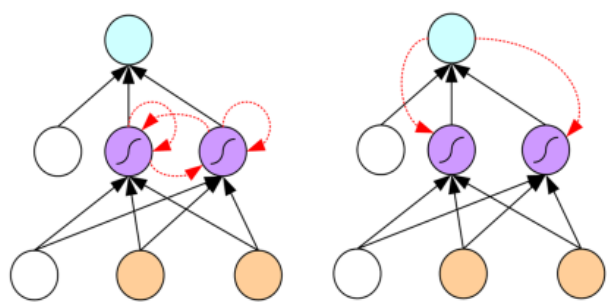
\includegraphics[width=7cm]{rnn.png}
		\caption{RNN architecture.}
		Traditional RNNs of Elman-Type (left) and Jordan-Type (right). Source: \cite{mesnil:2015}.
		\label{fig:rnn}
	\end{center}
\end{figure}

A common solution to this problem comes in the form of so called Long Short Term Memory (LSTM) networks. These special type of RNNs consist of several layers interacting in a certain way so that information can flow along it unchanged. This allows gradients to flow nicer over time. In detail, a LSTM-module consists of an \textit{input-gate} $i$, a  \textit{forget-gate} $f$ and an \textit{output-gate} $o$, as well as a memory cell $c$ and a hidden state $h$. Their values at timestep $t$ are computed as follows (see \cite{zhai:2017}):
\begin{eqnarray*}
	i_t	&=&	\sigma(W^i x_t + U^i h_{t-1} + b^i)\\
	f_t	&=&	\sigma(W^f x_t + U^f h_{t-1} + b^f)\\
	o_t	&=&	\sigma(W^o x_t + U^o h_{t-1} + b^o)\\
	g_t &=& \tanh(W^g x_t + U^g h_{t-1} + b^g)\\
	c_t &=&	f_t \otimes c_{t-1} + i_t \otimes g_t\\
	h_t &=& o_t \otimes \tanh(c_t)
\end{eqnarray*}
Hereby, $\otimes$ denotes element-wise multiplication, $\sigma(\cdot)$ is the element-wise sigmoid-function and $\tanh(\cdot)$ the element-wise hyperbolic-tangent function. Also $W^i, W^f, W^o, W^g U^i, U^f, U^o$ and  $U^g$ are shared weight-matrices and $b^i, b^f, b^o$ and $b^g$ are shared bias-vectors.
A diagram illustrating the function of such a module is illustrated in figure \ref{fig:lstm}. Because of their ability to capture long-term dependencies very well, LSTMs or similar modules such as \textit{Gated Recurrent Units} (GRU) (see for example \cite{zhang:2016}) have been the preferred choice for many researchers of NLU in recent years (\cite{kurata:2016}, \cite{ravuri:2015}, \cite{yang:2016}, \cite{zhai:2017}, \cite{zhang:2016})

\begin{figure}[H]
	\begin{center}
		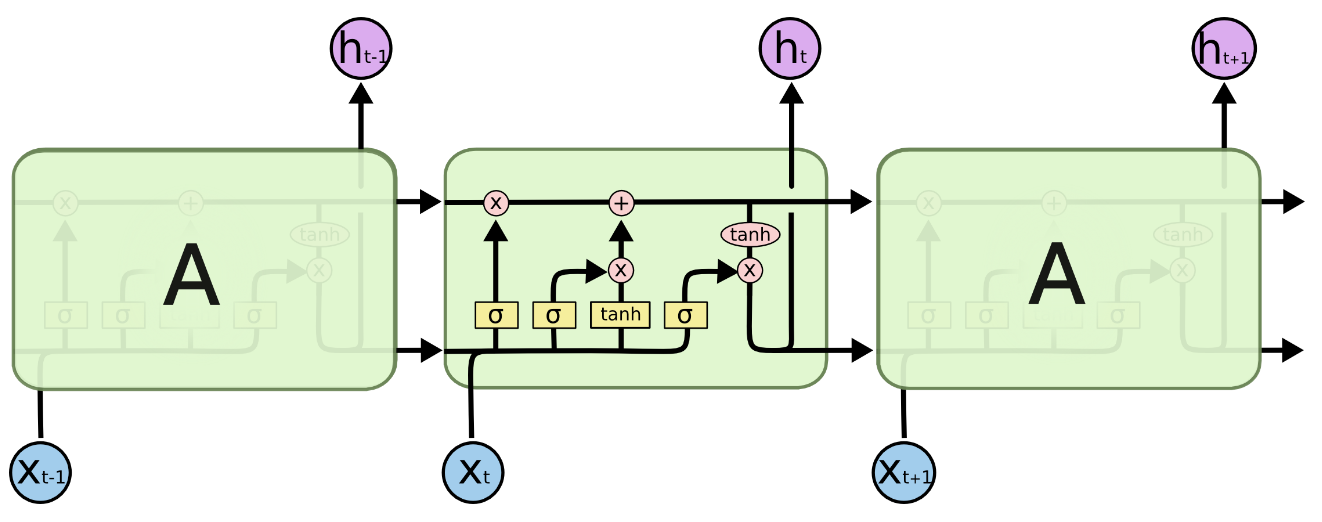
\includegraphics[width = 14cm]{lstm.png}
		\caption{LSTM-Module.}
		Source: http://colah.github.io/posts/2015-08-Understanding-LSTMs/.
		\label{fig:lstm}
	\end{center}
\end{figure}

\subsection{Bidirectional LSTMs}
Since in the task of NLU we have the full sentence at our disposal before starting the classification, instead of only encoding information about the previous words $x_1, \dots, x_{t-1}$ of $x_t$ into the LSTM, we can also go backwards through the sentence to encode information about the following words $x_{t+1}, \dots, x_T$. To account for information about the whole sentence when computing the hidden-state for the word $x_t$, we can combine these two approaches to a so called \textit{bi-directional} LSTM (Bi-LSTM): First, the word-sequence $x_1, \dots, x_T$ gets run through the LSTM to compute hidden-states $\overrightarrow{h_1}, \dots, \overrightarrow{h_T}$. Then, the word-sequence again gets run through the LSTM but in reverse order $x_T, \dots, x_1$ to compute hidden-states $\overleftarrow{h_T}, \dots, \overleftarrow{h_1}$. The hidden-state $\overleftrightarrow{h_t}$ of the Bi-LSTM at time-step $t$ is then generated as the concatenation $\overleftrightarrow{h_t} = [\overleftarrow{h_t}, \overrightarrow{h_t}]$ (c.f. \cite{yang:2016},\cite{zhai:2017}).

\subsection{Convolutional Neural Networks}
Another tool that is used in the model of \cite{zhai:2017} are \textit{Convolutional Neural Networks}  to compute feature vectors for each chunk to use for labeling. In this article we will not explain CNN-architecture in detail (for that see for example \cite{kim:2014}), just briefly how it is used: a CNN with $m$ filters and a filter-size of $n$ (and a stride of $1$) is used to compute $m$-dimensional feature-vectors for each $n$-gram in the chunk. Afterwards a max-pooling-layer over all of these feature-vectors gets us a single feature-vector for the whole chunk that can be used for labeling.\par
By using a CNN for feature-extraction we don't have to be concerned about the number of words in each chunk and instead have a single feature-vector of fixed size.

\subsection{Pointer Networks}
\label{sec:ptrnets}
In the model, the chunks will be identified in a greedy way, i.e. one chunk after the other. Since all chunks are adjacent, this means we will only ever have to identify the end-point of the next chunk because the start is given by the end-point of the last one. This behaviour can be realized by the use of so called \textit{Pointer Networks} (PN) which were proposed by Vinyals et al. in \cite{vinyals:2015}. The goal of a PN is to match sequences $\mathcal{P} = \lbrace P_1, \dots, P_n \rbrace$ of vectors to sequences of indices $\mathcal{C}^\mathcal{P} = \lbrace C_1, \dots, C_m \rbrace \subseteq \underline{n}^m$ of these vectors, i.e. \textit{pointers} to vectors in $\mathcal{P}$. The probability of a pointer-sequence $\mathcal{C}^\mathcal{P}$ given $\mathcal{P}$ is calculated as
\[
	p(\mathcal{C}^\mathcal{P} \vert \mathcal{P}) = \prod_{i=1}^m p(C_i \vert C_1, \dots, C_{i-1}, \mathcal{P})
\]
so Vinyals et al. designed a parametric model (a RNN with parameters $\theta$) to estimate the terms of the product
\[
	p_\theta (C_i \vert C_1, \dots, C_{i-1}, \mathcal{P};\theta) \approx p(C_i \vert C_1, \dots, C_{i-1}, \mathcal{P}).
\]
To estimate this probability they proposed an encoder-decoder-framework, i.e. using one \textit{encoder}-RNN that runs over $\mathcal{P}$ to produce a hidden-state sequence $e_1, \dots, e_n$, whose final hidden state $e_n$ is then used to initialize a second \textit{decoder}-RNN that produces the sequence $d_1, \dots, d_m$ of states. They then calculated the probability via
\begin{eqnarray*}
	u_j^i	&=&	v^{tr} \tanh(W_1 e_j + W_2 d_i)	\quad\quad \text{for } j \in \lbrace 1, \dots, n\rbrace\\
	p_\theta(C_i \vert C_1, \dots C_{i-1}, \mathcal{P}; \theta) &=& \text{softmax}(u^i)
\end{eqnarray*}
Hereby $W_1, W_2$ and $v$ as well as the parameters of the decoder and the encoder-RNN are trainable. A visualization of the PN is given in figure \ref{fig:ptrnet}.\par
We can now easily see how the concept of PNs applies to the problem of identifying chunks: the sequence $\mathcal{P}$ becomes our input-word-sequence and the index-sequence $\mathcal{C}^\mathcal{P}$ is the sequence of start/end-points of the chunks. How exactly PNs are applied in the chunking model will be explained in the next section.

\begin{figure}
	\begin{center}
		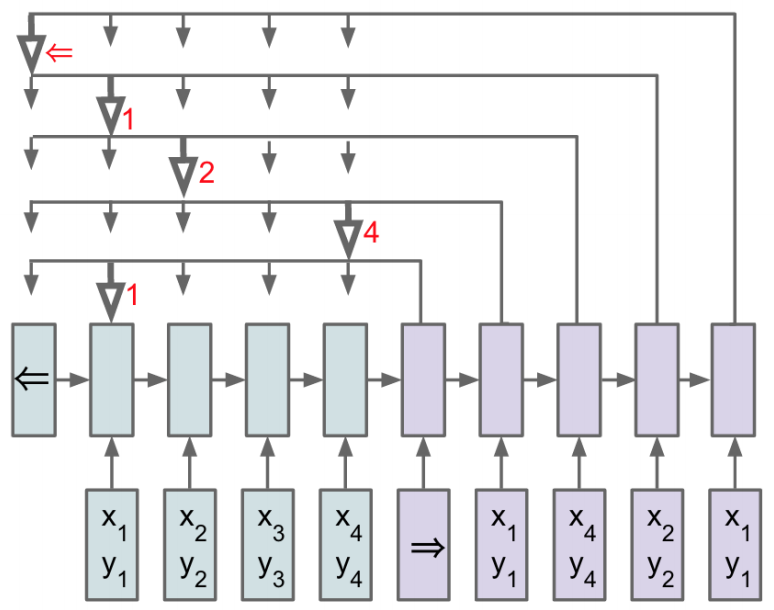
\includegraphics[width=7cm]{ptrnet.png}
		\caption{PN architecture.}
		The input-sequence is first encoded with an encoder-network (blue) to initialize the decoder-network (purple). The outputs of the decoder are then used to point to one of the input-words via softmax. Source: \cite{vinyals:2015}.
		\label{fig:ptrnet}
	\end{center}
\end{figure}


\subsection{The Model}

Now that we have explained all tools needed, we will describe the full model of Zhai et al. \cite{zhai:2017} in detail. Note that some of the notation was changed to make for better consistency.\\
\ \par
The model follows an encoder-decoder framework similar to the one described in section \ref{sec:ptrnets}. We have an encoder-network in the form of a Bi-LSTM and a decoder-network in the form of a usual LSTM. After the whole sentence is encoded, the information is used to greedily identify semantic chunks with a PN which are then immediately used as input to the decoder. The output of the decoder is used for labeling the current chunk.\par
The encoder uses word-embeddings $(E x_1, \dots, E x_T)$ of the words $(x_1, \dots, x_T)$ of the input sequence, which are provided in \textit{one-hot-representation} (i.e. vectors of size $\vert V \vert$ with a $1$ at the correct index and $0$'s otherwise) and produces the hidden-state sequence $\overleftrightarrow{h_1}, \dots, \overleftrightarrow{h_T}$ for a matrix $E \in \mathbb{R}^{m \times \vert V \vert}$. The sentence-representation $[\overrightarrow{h_T}, \overleftarrow{h_1}]$ (i.e. the concatenation of the final hidden states of the forwards- and of the backwards-LSTM) is used to initialize the decoder-LSTM, together with an special starting input token. The process of continually identifying chunks and labeling them now works as follows:\\
\ \par
For a chunk beginning at time step $b$ (for the first chunk this is the start of the sentence, for later chunks the beginning is set at the end of the previous chunk) the probabilities of all possible endpoints are calculated in a way that is similar to the Pointer Networks from section \ref{sec:ptrnets}. First, we define the vector
\[
	u_j^i = v_1^{tr} \tanh(W_1 \overleftrightarrow{h_j} + W_2 E x_j + W_3 E x_b + W_4 d_i) + v_2^{tr} LE(j-b+1)
\]
with $j \in \lbrace b, \dots, b+l_m-1 \rbrace$. Here, $i$ is the index of the chunk, $v_1$ and $v_2$ are trainable vectors, $W_1, W_2, W_3$ and $W_4$ trainable matrices, $l_m$ is a hyperparameter for the maximum chunk length and $LE(j-b+1)$ is a chunk-length embedding that is not precisely specified in \cite{zhai:2017} but is also a trainable parameter. This is comparable to the feature-vector for PNs but instead of only having the encoder hidden-state $\overleftrightarrow{h_j}$ and the previous decoder hidden-state $d_i$ as the input, we add the word embeddings of the beginning word $x_b$ and the word at the current position $x_j$, as well as an embedding for the length of the chunk. Now the probabilities of chunk $i$ ending at position $j$ are given by
\[
	p_i(j) = \frac{exp(u_j^i)}{\sum_{k=b}^{b+l_m-1} exp(u_k^i)},
\]
i.e. $p_i \equiv softmax(u^i)$. The ending point $e$ can now be greedily chosen as the point with maximum probability
\[
	e := \underset{j \in \lbrace b, \dots, b+l_m-1 \rbrace}{\text{argmax}} (p_i(j)).
\]\\
\ \par
After identifying the scope of the chunk, it will now be used to compute the input $C_{i+1}$ to the decoder for the next time-step. This input consists of several parts:

\begin{itemize}
	\item First, we compute the feature extraction of the current chunk via a CNN:
		\[
			C_{i+1,x} := g(E x_b, \dots, E x_e) 
		\]
		where $g(\cdot)$ gives us the output of the CNN (in the paper \cite{zhai:2017}, this step is depicted with using the $x_j$ directly as input to the CNN but this is presumably inaccurate, or the embedding was included in $g$).
	\item Second, we compute a representation of the hidden states of the encoder for the words in the chunk by
		\[
			C_{i+1,h} := \text{Average}(\overleftrightarrow{h_b}, \dots, \overleftrightarrow{h_e})
		\]
	\item Third, we use a context-window to capture context information for the chunk. With context-window size $d$ (which is a tunable hyperparameter) this means
		\[
			C_{i+1,w} := [ A x_{b-d}, \dots, A x_{b-1}, A x_{e+1}, \dots, A x_{e+d}]
		\]
		is the concatenation of the $d$ words preceeding and the $d$ words following chunk $i$.
	\item Now $C_{i+1} := [C_{i+1,x}, C_{i+1,h}, C_{i+1,w}]$ is the concatenation of the three components.
\end{itemize}
The output of the decoder can be used for labeling, for example if the outputs are viewed as probabilities for the slot labels via a softmax-layer, we can assign the label with maximum probability.\\
\ \par
A diagram depicting the model can be found in figure \ref{fig:model3}.

\begin{figure}
	\begin{center}
		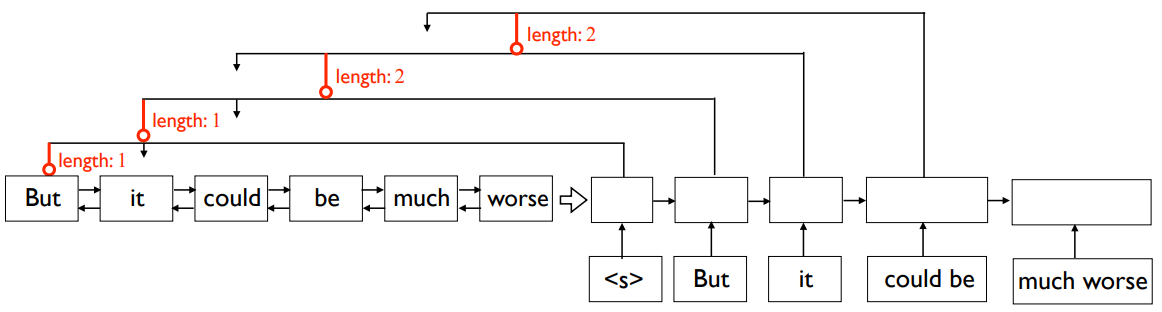
\includegraphics[width = 15cm]{model3.png}
		\caption{Encoder-decoder-pointer framework.}
		The presented framework used on the example sentence \textit{'But it could be much worse'}. On the left is the encoder-BiLSTM, which is used to encode the sentence for the decoder-LSTM on the right. Inputs to the decoder are the chunks identified in the previous timestep. A PN with a maximum chunk length of $2$ calculates the probabilities of the possible ending points. The chosen ending point is pointed to in red color. Source: \cite{zhai:2017}.
		\label{fig:model3}
	\end{center}
\end{figure}

\subsection{Training criterion}
Since the task essentially is split into two subtasks which are solved simultaneously (segmentation and labeling), there are also two loss functions to be considered. Zhai et al. used the sum of the cross-entropy loss for both subtasks as loss function for the whole model:
\[
	L(\theta) := L_{\text{segmentation}}(\theta) + L_{\text{labeling}}(\theta)
\]
where $L_{\text{segmentation}}(\theta)$ is the cross-entropy loss for the segmentation task and $L_{\text{labeling}}(\theta)$ the cross-entropy loss for the labeling task with trainable parameters $\theta$. The model is then trained by stochastic gradient descent on the loss function $L(\theta)$.

\subsection{Performance on Slot Filling task}
In this section we will describe, how well the model performed at the Slot Filling task of NLU. Zhai et al. also reported the performance on the sequence chunking task but since this is not as relevant for NLU we will omit these results for now.\par
The performance was evaluated on two different datasets:
\begin{itemize}
	\item The \textit{Airline Travel Information System} (ATIS) corpus. This dataset consists of $4,978$ training and $893$ test sentences from the airline travel domain. It has a vocabulary size if $572$ and contains $84$ different slot-labels ($127$ if counting IOB prefixes). This dataset is widely regarded as one of the standard datasets for evaluating NLU performance and thus has been used by many researches (e.g. in \cite{goo:2018}, \cite{kurata:2016}, \cite{mesnil:2015}, \cite{mesnil:2013}, \cite{ravuri:2015}, \cite{yao:2013}, \cite{zhai:2017},  \cite{zhang:2016}). For more information on how this dataset was collected and transcribed, see \cite{hemphill:1990}.
	\item A larger dataset (LARGE) prepared by merging the ATIS corpus with the MIT Restaurant Corpus and the MIT Movie Corpus \cite{liu:2013a} \cite{liu:2013b}. In total this large dataset contains $30,229$ training and $6,810$ testing sentences. The vocabulary size is $16,049$ and the number of slot labels is $116$ ($194$ if counting IOB prefixes). This dataset is obviously much larger than the ATIS dataset and has three different domains so it poses more of a challenge. However it is not as widely used so there are few other models to compare the score on this dataset to (we only compare to \cite{kurata:2016}).
\end{itemize}
The performance is measured by the $F_1$-Score which is the harmonic mean of \textit{Precision} and \textit{Recall} value:
\[
	F_1 = \frac{2 \times Precision \times Recall}{Precision + Recall}
\]
where
\[
	Precision = \frac{\# \text{correctly labeled words}}{\# \text{total labeled words}}
\]
and
\[
	Recall = \frac{\# \text{correctly labeled words}}{\# \text{words with nonempty label as ground truth}}
\]
(\cite{rijsbergen:1979}). The best possible score is $1$ (perfect labeling) and the worst is $0$ (no correct label). This $F_1$ score is commonly used for evaluating classification tasks. Table \ref{tab:f1} shows the $F_1$ score of the presented model compared to different Neural Network based  models from some other papers of the past few years on the ATIS and the LARGE dataset.

\begin{table}[H]
	\begin{center}
		\begin{tabular}{|l|c|c|}
			\hline
			Model															&ATIS $F_1$	&LARGE $F_1$\\ \hline \hline
			Bi-dir. Jordan RNN (Mesnil et al., 2013) \cite{mesnil:2013}	&$93.98\%$	&- \\ \hline
			RNN (Yao et al., 2013) \cite{yao:2013}							&$94.11\%$	&- \\ \hline
			Hybrid RNN (Mesnil et al., 2015) \cite{mesnil:2015}			&$95.06\%$	&- \\ \hline
			Slot Gated (Goo et al., 2018) \cite{goo:2018}					&$95.20\%$	&- \\ \hline
			Joint ID + SF (Zhang et al., 2016) \cite{zhang:2016}			&$95.49\%$	&- \\ \hline
			Enc.-Dec. LSTM (Kurata et al., 2016) \cite{kurata:2016}		&$95.66\%$	&$74.41\%$ \\ \hline
			\textbf{Sequence Chunking (Zhai et al., 2017)} \cite{zhai:2017})&$\textbf{95.86\%}$	&$\textbf{78.49\%}$ \\ \hline
		\end{tabular}
		\caption{$F_1$-Score comparison of different models on ATIS and LARGE dataset}
		\label{tab:f1}
	\end{center}
\end{table}

As we can see from table \ref{tab:f1}, the presented sequence chunking model by Zhai et al. produces state of the art results and stands as one of the most successful models for the Slot Filling task today.

%%%%%%%%%%%%%%%%%%%%%%%%%%%%%%%%%%%%%%%%%%%%%%%%%%%%%%%%%%%%%%%%%%%%%%%%%%%%%%%
%
%
%               Section 4 - Models for Intent Determination
%
%
%%%%%%%%%%%%%%%%%%%%%%%%%%%%%%%%%%%%%%%%%%%%%%%%%%%%%%%%%%%%%%%%%%%%%%%%%%%%%%%
\section{Models for Intent Determination}

%%%%%%%%%%%%%%%%%%%%%%%%%%%%%%%%%%%%%%%%%%%%%%%%%%%%%%%%%%%%%%%%%%%%%%%%%%%%%%%
%
%
%               Section 5 - Joint models for multiple subtasks
%
%
%%%%%%%%%%%%%%%%%%%%%%%%%%%%%%%%%%%%%%%%%%%%%%%%%%%%%%%%%%%%%%%%%%%%%%%%%%%%%%%
\section{Joint models for multiple subtasks}

%%%%%%%%%%%%%%%%%%%%%%%%%%%%%%%%%%%%%%%%%%%%%%%%%%%%%%%%%%%%%%%%%%%%%%%%%%%%%%%
%
%
%               Section 6 - Conclusion
%
%
%%%%%%%%%%%%%%%%%%%%%%%%%%%%%%%%%%%%%%%%%%%%%%%%%%%%%%%%%%%%%%%%%%%%%%%%%%%%%%%
\section{Conclusion}


\newpage
\addcontentsline{toc}{section}{References}
\bibliographystyle{plain}
\bibliography{quellen}

\end{document}
